% (C) Anders Kofod-Petersen
\documentclass[a4paper,norsk,oneside]{book}
\usepackage[norsk]{babel}						% Correct English hyphenation
\usepackage[utf8]{inputenc}						% Allow for non-English letters
\usepackage{graphicx}							% To include graphics
%\usepackage{natbib}								% Correct citations
%\usepackage{fancyheadings}						% Nice header and footer
\usepackage[linktocpage,colorlinks]{hyperref}			% PDF hyperlink
\usepackage{geometry} 							% Better geometry
%\usepackage[center]					% For cropping documents
\usepackage{url}
\usepackage{float}
% B5 (uncomment to convert to B5 format)
 \geometry{b5paper}

% Author
% Fill in here, and use commands in the text. 
\newcommand{\thesisAuthor}{Geokomai}
\newcommand{\thesisTitle}{Prosjektrapport }
\newcommand{\thesisType}{Eksperter i Team}
\newcommand{\thesisDate}{Vår 2013}

% PDF info
\hypersetup{pdfauthor={\thesisAuthor}}
\hypersetup{pdftitle={\thesisTitle}}
\hypersetup{pdfsubject={\thesisType}}
\hypersetup{linkcolor=black}
\hypersetup{citecolor=black}
\hypersetup{urlcolor=black}

%Fancy headings
%\pagestyle{fancy}
%\pagestyle{fancyplain}
%\renewcommand{\chaptermark}[1]{\markboth{#1}{}}
%\renewcommand{\sectionmark}[1]{\markright{#1}{}}
%\lhead[\fancyplain{}{\thepage}]{\fancyplain{}{\let\uppercase\relax\leftmark}}
%\rhead[\fancyplain{}{\let\uppercase\relax\rightmark}]{\fancyplain{}{\thepage}}
%\chead[\fancyplain{}{}]{\fancyplain{}{}}
%\lfoot[\fancyplain{}{}]{\fancyplain{}{}}
%\cfoot[\fancyplain{}{}]{\fancyplain{}{}}
%\rfoot[\fancyplain{}{}]{\fancyplain{}{}}

% Citation format
%\bibliographystyle{apalike}
%\bibpunct{[}{]}{;}{a}{,}{,}

\begin{document}

%Title page (This is generate automatically from the commands above)
\begin{titlepage}
\noindent {\large \textbf{\thesisAuthor}}
\vspace{2cm}

\noindent {\Huge \thesisTitle}
\vspace{2cm}

\noindent \thesisType, \thesisDate 
\vspace{2cm}

%\noindent Artificial Intelligence Group\\ Department of Computer and Information Science\\ Faculty of Information Technology, Mathematics and Electrical Engineering\\

\vfill
\begin{center}

\includegraphics[width=3cm]{figs/NTNUlogo.pdf}
\end{center}
\end{titlepage}

\thispagestyle{empty}

\cleardoublepage

\frontmatter

\section*{Abstrakt}

I dag finnes det en rekke applikasjoner og tilgjengelig informasjon relatert til vei, veiforhold, navigasjon, kart, trafikkmeldinger og lignende. Tjenesten Google Maps er nok for mange et kjent fenomen, som er en web-basert applikasjon for kart og navigasjon. Det er også flere kilder som tilbyr informasjon i forbindelse med både trafikkmeldinger og værdata, som for eksempel vegvesenet og yr.no. Alt dette er viktige faktorer for å kunne avgjøre om en reiserute er trygg og effektiv, og det er nettopp dette vi vil belyse i denne oppgaven. Prosjektet vårt går ut på å samordne eksisterende kilder til sanntidsinformasjon til et integrert intelligent system som kan ta beslutninger om hvilke reiseruter som er tryggest og mest effektive for veiferdsel. Den store utfordringen vil være å samordne informasjon og data fra flere forskjellige kilder, som igjen kan danne et grunnlag for å presentere dette på en enkel plattform.

%\begin{itemize}
%\item the field of research
%\item a brief motivation for the work
%\item what the research topic is and
%\item the research approach(es) applied. 
%\item contributions
%\end{itemize}



\clearpage

\section*{Forord}



\vspace{1cm}

Denne rapporten leveres som en del av faget TDT4853 - “Eksperter i Team” ved Norges Tekniske-Naturvitenskapelie Universitet (NTNU), våren 2013. Gruppen Geokomai har utarbeidet rapporten under landsbyen “Det intelligente transportsystemet”. 

Vi vil rette en takk til:
\begin{itemize}	
\item Pauline Haddow, landsbyleder
\item Eivind Myklebust Lindseth, studentassistent
\item Edel Gustavsen Holand, studentassistent
\end {itemize}




\vfill

\hfill \thesisAuthor

\hfill Trondheim, \today

\clearpage

\tableofcontents

\listoffigures

\listoftables

\mainmatter

\chapter{Innledning}
\label{cha:Introduction}
Gruppen Geokomai består av seks studenter med ulik bakgrunn og kompetanse. To av studentene går Datateknikk, med spesialisering innenfor Intelligente Systemer, og studenten som går Informatikk har også sin fordypning innenfor samme felt. En av gruppmedlemmene 
går Kommunikasjonsteknologi med fordypning innen Nett og Tjenester, den femte studenten har sin bakgrunn innenfor Teknisk Geofag, mens sistemann har Geomatikkompetanse. Den største kontrasten ligger nok mest innenfor de to sistnevnte, da Datateknikk og Kommunikasjonsteknologi er to linjer som har mye til felles. Ved valg av prosjektoppgave hadde vi i startfasen vanskeligheter med å finne en problemstilling som dekket alles felt. Men etter hvert som samordning av ulike kilder og data ble et alternativ, fant vi fort ut av at utformingen og arbeidet rundt vår applikasjon vil ha såpass mye bredde, at alles kompetanse ville spille en rolle.

Vårt applikasjonskonsept skal være til hjelp for reisende og vise nyttig informasjon.  Denne informasjonen kan være for eksempel sanntidsinformasjon for værdata, trafikkmeldinger, trafikkuhell, trafikktetthet, ras, fergeavganger og tilsvarende. Målet er å koordinere informasjon fra flere forskjellige kilder, og prosjektet vil ta for seg hvilke kilder som er mest relevante. Trafikkmeldinger om trafikkflyt,  trafikkonsentrasjon fra NVDB og vegvesenet, veibaneforhold fra yr.no, historiske viltpåkjørsler fra Direktoratet for naturforvaltning. Ras og flomutsatte veistrekninger fra NVE i samarbeid med vegvesenet og Metrologisk Institutt.
	
Når data er samlet vil det bli undersøkt hvordan det bør presenteres til brukeren på en oversiktlig måte. Målet er å filtrere informasjonen og bare vise informasjon som er relevant for den gjeldende brukeren, basert på for eksempel posisjon og rute. Vi ønsker å presentere brukeren en risikoprofil for den veistrekningen de befinner seg på i sanntid.

Denne rapporten vil være et forarbeid til en slik applikasjon, og målet er å undersøke hvilke informasjonskilder som finnes og hvordan disse kan integreres til en felles løsning. Sluttresultatet vil være en rapport med forslag til et brukergrensesnitt. 

\chapter{ Analyse av eksisterende løsninger}\label{T-B}
\label{cha:TheoryAndBackground}

{\it I dag finnes det en rekke applikasjoner relatert til vei og transport. Disse løsningene viste seg å generelt sett være spesifikke mot et problemområde, men enkelte var også mer komplette løsninger. Vi har valgt å se nøyere på løsningene som er mest relevante for vår applikasjon og finne ut av om disse kan være til hjelp og inspirasjon for vårt konsept, ikke minst om de er mangelfulle og har et forbedringspotensiale.}


\section{Norske løsninger}
\label{sec:no1}

Det norske markedet for applikasjoner som hjelper deg på reise er ikke like modent som det internasjonale markedet. Ingen enerådende løsninger finnes, men vi har sett på 14 applikasjoner i det norske markedet. Disse applikasjonene finnes enten i Google Play, Apple App Store eller som enkeltstående webapplikasjoner.

Crowdsourcing er blitt populært for å samle inn informasjon fra brukere, og internasjonalt har flere applikasjoner gjort god nytte av dette. Vi undersøkte og kom frem til at brukermassen i Norge ikke er stor nok til at disse får noen særlig nytteverdi. Ingen norske løsninger benytter seg av denne teknologien. NRK P4s applikasjon viser informasjon fra innringte trafikkmeldinger, og det er mulig å registrere en trafikkulykke eller kø. Dette er det nærmeste man har vellykket crowdsourcing i det norske markedet.

Tilgangen på trafikkdata i Norge begrenser funksjonaliteten til applikasjonene, og de fleste appene benytter seg av de samme dataene. Dataene som er tilgjenglige er:

\begin{itemize}
\item Trafikkmeldinger fra Statens veivesen, Trafikksentralen
\item Bilder fra veikameraene til Statens veivesen
\item Data om trafikktetthet på teststrekninger fra Statens veivesen
\end{itemize}
Underveis i prosjektet åpnet vegvesenet Norsk veidatabank (NVDB) for bruk i applikasjoner, og datatilgangen har derfor forbedret seg, som vi skal se på senere i rapporten, men applikasjonsutviklere har ikke hatt tid til å utnytte disse dataene i stor grad.

Alle applikasjonene er svært like, og lite skiller de fra hverandre. Dette bunner ut fra den samme begrensede tilgangen på data. De viser trafikkmeldingene fra SVV på et kart, med noe tilhørende metadata. Vi konkluderer dermed med at det ikke finnes noen komplett reiseassistent-applikasjon i Norge.

Undersøkte applikasjoner:

\begin{itemize}
\item Trafikk - av NAF og VG
\item iTrafikken - Ciber Norge AS
\item Trafikk Melding - Trafikkinfo
\item Trafikkflyt - P4
\item Traffikkflyt Bergen
\item Trafikk - Frank Burmo
\item Trafikk Widget - Unixcrap Apps
\item veiAppen - Sveinung Kval Bakken
\item Statoil
\item Trafikkmelding
\item Dit.no
\item Google Maps
\item Apple Maps
\end{itemize}

Applikasjonene finnes på Google Play eller Apple App Store

%
%\begin{itemize}
%\item when referring to authors:\\
% \citet{authorson10:_secon_best_paper_in_world} stated something rather nice.
%\item to cite indirectly: \\
% Papers should be written nicely \citep{authorson10:_secon_best_paper_in_world}\\
%or\\
%In \cite{authorson10:_secon_best_paper_in_world}, a less detailed template was presented.
%\item To just cite the authors: \\
%\citeauthor{authorson10:_secon_best_paper_in_world} wrote a nice paper.
%%\item Or just the year: \citeyear{authorson10:_secon_best_paper_in_world}.
%%\item You can even cite specific pages: \citet[p. 3]{authorson10:_secon_best_paper_in_world}.
%\end{itemize}
%
%\vspace{0.5cm}
%
%\noindent
%{\bf Introducing figures:} \\

%\begin{figure}[ht]
%\begin{center}
%\includegraphics[width=0.5\columnwidth]{figs/figure1.pdf}
%\caption[Boxes and arrows are nice]{Boxes and arrows are nice (adapted from \citet{authorson10:_secon_best_paper_in_world})}
%\label{fig:BoxesAndArrowsAreNice}
%\end{center}
%\end{figure}

%Remember that when you borrow figures you should always credit the original author --- such as Figure \ref{fig:BoxesAndArrowsAreNice} (adapted from \citet{authorson10:_secon_best_paper_in_world}). Also don't just put the figure in and leave it to the author to try to understand what the figure is. The figure should be put in to convey a message and you need to help the author to understand the message intended by explaining the figure in the text. 

%\vspace{0.5cm}
%
%\noindent
%{\bf Introducing tables in the report: }\\
%
%\begin{table}[htdp]
%\begin{center}
%\begin{tabular}{|c|c|c|c|c|}\hline\hline
%This & is & a & nice & table\\\hline
%This & is & a & nice & table\\\hline\hline
%\end{tabular}
%\caption{Example Table}
%\end{center}
%\label{tab:ExampleTable}
%\end{table}%

%As you can see from Table \ref{tab:ExampleTable}, tables are nice. However, again, you need to discuss the contents of the table in the text. You don't need to describe every entry but draw the authors attention to what is important for he/she to glean from the table. 

\section{Internasjonale løsninger}
I dette avsnittet vil vi se nærmere på det internasjonale markedet for trafikkapplikasjoner, for å undersøke om det finnes noe der ute vi kan bruke. Vi har prøvd å finne løsninger som tilbyr elementer av det vi ønsker å lage, og undersøkt om noe av det vi finner kan gjenbrukes i vår løsning. Fokuset ble spesielt lagt på det tekniske rundt applikasjonene og hvilke metoder de bruker for å samle inn informasjon knyttet til trafikken. Under følger en beskrivelse av de løsningene vi mener er de mest relevante innenfor forskjellige områder knyttet til vår problemstilling.

\subsection{Google Maps}
Google Maps kan beskrives som standarden innen kartløsninger, særlig på Internett. Tjenesten eksisterer både som en webløsning og som apper til de fleste mobile plattformer. En av funksjonene vi la spesielt merke til er muligheten for å vise sanntidsinformasjon fra trafikken. Google Maps viser trafikkmengden ved hjelp av fargekoder langs strekningen, og viser også eventuelle hindringer langs veien. Tjenesten tar hensyn til denne informasjonen når den regner ut hvilen rute som vil være raskest. I tillegg bruker den informasjonen til å estimere drivstofforbruk, ved å ta hensyn til rute, trafikkmengde og biltype.

(bilde)
Et eksempel på sanntidsdata hentet fra New York.
Gir informasjon om trafikkmengde, ulykker, veiarbeid, osv.

Sanntidsdataen blir hentet ved hjelp av anonym innsamling fra GPS-enheter som bruker veiene (en form for crowdsourcing). Google har et enormt brukergrunnlag tilgjengelig ved hjelp av Google Maps applikasjon til Android og iOS enheter. Sanntidsdata fra trafikken er kun utbredt tilgjengelig i de største landene som USA, Frankrike og Storbritannia. Nye land og byer legges til fortløpende. Sanntidsdata vises også i norske byer, men dette gjelder et veldig begrenset antall strekninger, og informasjonen virker ikke å være spesielt nøyaktig.

Google Maps tilbyr mange spennende funskjoner som lett kan tenkes å være en del av et intelligent trafikksystem. Spesielt integreringen av sanntidsdata og hvordan denne blir brukt er interessant for oss. Selv om mesteparten av disse funksjonene ikke er tilgjengelig i Norge, viser det oss at det er teknisk mulig å implementere de og gir oss tips om hvordan, ved f.eks bruk av crowdsourcing.

\subsection{Waze}
Waze er laget av et israelsk selskap og er en meget populær app som brukes over hele verden, men hovedsaklig i USA. All informasjon som leveres til brukeren er generert av andre brukere. Dette gjøres via en applikasjon til smarttelefoner, der man har mulighet til å rapportere ulike type hendelser, som f.eks. ulykker, fareelementer i veien og køer. Disse rapportene blir knyttet til veistrekningen man er på til en hver tid, og brukes til å advare andre trafikanter. 

Waze genererer både automatiske rapporter med bakgrunn i beveielsene til brukeren og manuelle rapporter som er lagt inn av brukere. De automatiske rapportene genereres ved å blant annet overvåke brukerens hastighet. Hvis man registrerer at brukeren forflytter seg saktere enn den gjeldende fartsgrensen på veien, vil det genereres en rapport om kø i dette området. Man har mulighet for å gi tilbakemelding på rapporter fra andre brukere, ved å enten godkjenne dem eller gi beskjed om at problemet ikke lenger er der. På denne måten vil trafikkmeldingene til en hver tid være oppdatert.

Waze har også mulighet til å sammenligne forskjellige ruter til en bestemt destinasjon. Den vil ta hensyn til rapporter om f.eks. kø og gi et estimat om hvor lang tid hver strekning vil ta. Waze har også innslag av intelligente funksjoner. Waze tilbyr mange spennende funksjoner og mange av dem kan inngå i vår løsning. Det som er spesielt interessant med Waze er alt innhold er generert av brukerene selv og at denne metoden er beviselig kapabel til å produsere et meget godt bilde av trafikken i sanntid.

\subsection{Ras}
Vi har forsøkt å finne løsninger i utlandet som kan vise rasfare langs en veistrekning uten å lykkes. Det finnes mange lokale informasjonssystemer, noen med tilhørende applikasjoner, som informerer om rasfare i spesielle områder. Dette gjelder helst snøskred og som oftest i forbindelse med skisentre. I tillegg virker som om de fleste av disse løsningene fokuserer på å oppgi risiko for ras i visse områder, og ikke informasjon om når det har gått et ras.

\subsection{Konklusjon}
Selv om det finnes mange nyttige applikasjoner internasjonalt knyttet til trafikk er vår oppfatning at ingen av dem tilbyr det totale pakken vi ser etter. Spesielt mangelfulle er løsninger som er knyttet til risiko i trafikken. Men det finnes mange gode løsninger der ute som tilbyr elementer av det vi ønsker å integrere i løsningen vår. Det bredeste utvalget finnes innen ruteplanlegging og presentasjon av sanntidsdata fra trafikken. Her er det mye vi kan ta med oss videre, og da spesielt ved å undersøke hvordan disse applikasjonene samler inn data.

\chapter{Analyse av eksisterende datakilder}
\label{sec:datakilderl}
{ \it Mangler en introduksjon til kapittelet her} 

\section{Vei}
For å kunne advare brukere om hindringer langs den ruten de kjører på er vi avhengig av å kunne hente informasjon om f.eks. ulykker, stengte veier, osv. Den beste kilden til slik informasjon fant vi gjennom vegvesenet som tilbyr en tjeneste kalt Trafikkmeldinger. Nærmest samtlige trafikkapplikasjoner som finnes i Norge henter data fra denne kilden. Disse meldingene tilbyr informasjon om blant annet ulykker, stengte veier og redusert fremkommelighet. Alle meldingene har knyttet til seg metadata som navnet på veistrekningen, veinummeret, posisjonen hvor hendelsen er rapportert. Dette vil gjøre det enklere for oss å filtrere informasjonen og kun presentere relevant informasjon til brukeren. Dataene kan hentes ut via et API i-XML format på veivesenets hjemmesider. Dataene kan også sorteres på fylke, slik at man kun får opp resultater fra der man er.

I tillegg til sanntidsdata trenger vi tilgang til historiske data for ulykker for å lage risikoprofilen. Norsk veidatabank(NVDB) tilbyr slik data, som er tilgjengelig via et eget API, der dataen kan hente ut data i både XML og JSON format. En av svakhetene med denne informasjonen er at ulykker uten personskade ser ut til å registreres sjeldent i NVDB. Det hadde vært fordelaktig å ha en oversikt over mindre ulykker også, for å kunne gi mer data til risikoprofilen. Det finnes et prøveprosjekt mellom Falck og vegvesenet, der man også registrerer mindre ulykker, som utforkjørsler uten personskade samt data rundt disse. Dette er dessverre ikke data som er tilgjengelig for publikum. Selv om det ikke er tilgjengelig per i dag kan det bli det i fremtiden.

Dette er et område der crowdsourcing kan være et nyttig hjelpemiddel. Som tidligere nevnt har vi observert at crowdsourcing er brukt i utlandet med gode resultater som verktøy til å rapportere om nettopp slik informasjon, og vi mener at dette bør være mulig også i Norge. Informasjonen som samles inn ved hjelp av crowdsourcing kan koordineres med data fra blant annet vegvesenet, slik at vi kan presentere så nøyaktig informasjon som mulig. 

\section{Værdata}
For å kunne forutse forholdene langs en rute med en viss nøyaktighet er vi avhengige av å hente ut presise værvarsler for steder langs ruten og nærliggende områder. Hvis det for eksempel er meldt kraftige regnbyer i et særlig flomutsatt område langs ruten, er sannsynligheten høy for overflatevann og flom. Da må vår applikasjon være istand til å forutse dette og gi brukeren en advarsel om den potensielle faren. Været har åpenbart stor innvirkning på mange av de fareelementene vi leter etter, derfor er det essensielt å finne en kilde til værdata som er så nøyaktig som mulig. Vær og vind kan endre seg fort, og vi er derfor også avhengig av kunne hente værdata som til en hver tid er oppdatert etter gjeldende forhold. De viktigste kravene vi setter til en slik kilde er derfor at vi må kunne hente nøyaktig og oppdatert informasjon ned til et visst nivå. Med tanke på at vi lager en applikasjon til smarttelefoner er det også ønskelig å kunne hente ut informasjon basert på gjeldende GPS posisjon, da denne informasjonen er lett tilgjengelig i slike applikasjoner. Værdata internasjonalt er gjerne samlet inn av private selskaper og solgt til de som er interessert. I Norge er man derimot så heldig at kan man finne gratis tilgjengelig data fra flere kilder. Vi tatt en nærmere titt på 3 forskjellige kilder, yr.no, storm.no og Meterologisk Institutt.

\subsection{Yr.no}
Yr.no har tilgjengeliggjort all sin data via et åpent API, som gjør at hvem som helst kan hente data herfra. Det finnes visse restriksjoner på hvor ofte man kan hente ut data, men dette begrenser ikke vår eventuelle bruk av tjenesten. Tjenesten fungerer ved at man sender inn en lokasjon og får tilbake en værmelding for denne lokasjonen. En annen nyttig funksjon yr.no tilbyr er informasjon om værforhold ved fjelloverganger, som jo kan være nyttig når man skal over en av disse. Et negativt aspekt ved yr.no er at det ikke er mulig å hente værvarsler basert på GPS posisjoner, men heller stedsnavn.

\subsection{Meteorologisk institutt}
Meterologisk institutt tilbyr mye de samme dataene som yr.no, og har også et eget API man kan kommunisere med.\cite{met} Forskjellen er at Meterologisk Institutt tilbyr større mengder data som i tillegg er mer detaljerte. Her kan man hente ut informasjon om alt fra skogbrannsfare til bølgehøyde i tillegg til detaljerte værvarsler. Man kan til og med hente hvor stor sannsynligheten for at et gitt værvarsel slår til. Informasjonen som er tilgjengelig er hentet fra værstasjoner som er plassert rundt om i Norge. Informasjonen er gjort tilgjengelig via et REST API og blir returnert i XML format.

\subsection{Storm.no}
Storm.no tilbyr dessverre ikke et åpent API for å hente ut data. De tilbyr derimot en tjeneste som ligner litt på det vi har tenkt å levere, nemlig trafikkvær. Her kan man planlegge en rute på et kart og få opp en værmelding langs denne ruten. På kartet er det også lagt inn veimeldinger. Vi kan dessverre ikke bruke denne tjenesten i vår applikasjon da det ikke er gjort tilgjengelig via et åpent API, men det viser at det er mulig og at det finnes interesse for slik informasjon blant det norske folk.
Det ble tidlig klart at Meterologisk Institutt var den kilden som passet våre behov best. Det tilbyr store mengder detaljerte data som er åpent og lett tilgjengelig via et REST API som enkelt kan kommunisere med vår tenkte applikasjon. I tillegg henter man informasjon basert på GPS posisjoner, noe som passer bra med tanke på at vi til en hver tid har tilgang til GPS posisjonen til brukeren gjennom bruken av smarttelefoner.

\section{Ras og Flom}
 Skred er en årsak til både forsinkelser og ulykker. Vi håper å kunne gi sjåføren en bedre og mer nøyaktig form for varsling av rasutsatte områder ved å hente oppdatert og tidsrelevant informasjon og analysere disse for brukeren. Skredfareskiltene som står langs veien tar ikke høyde for varierende risiko i ulike sesonger eller værforhold, og heller ikke typen skred, og det kan derfor være lett å ikke ta varslene på alvor av den grunn.
    Vi har sett på en del datakilder som er relevant for skred- og flomvarsling for å finne ut hva slags data de tilbyr, og hvor enkle disse er å ta i bruk for applikasjonsutviklere. Vi forventet å finne data om skred som har gått og blokkerer veibanen, samt vurdering av rasfaren i områdene som ligger langs veien. En epost-korrespondanse med en ansatt i NVE gjorde oss oppmerksom på at informasjon om skred som har gått er tilgjengelig hos vegvesenet. Vi har derfor justert forventningene våre, og ser etter datakilder som tilbyr rasfarevurdering og historiske data.
    Ras- og flomfare vil typisk være noe som gjelder for et stort område, og er ikke noe som kun er relevant for trafikken. Et par potensielle løsninger for å binde sammen datakilder vil være å enten kunne identifisere hvilken region en veistrekning tilhører, eller å identifisere hvilken region et koordinat tilhører. På denne måten kan man gå igjennom alle veistrekningene i en planlagt rute og finne rasfarevurderingen til disse basert på regionene de befinner seg i.
	Vi startet letingen etter datakilder på Norges Vassdrags- og Energidirektorat (heretter NVE), som tilbyr meget detaljerte kart på sine nettsteder for det meste innen ras og flom. (fotnote) Dessverre viste det seg fort at datatilgangen ikke var like god; foreløpig er det kun mulig å hente data om snøskredfare i 24 fjellområder rundt om i Norge. Da vi tok kontakt med NVE og stilte et par spørsmål rundt deres API-støtte fikk vi beskjed om at det var planer om å tilby jordskredfare og flomvarsling i løpet av sommeren 2013. NVE lar oss filtrere data etter regioner og koordinater og er derfor godt egnet for integrering i en applikasjon.
	Andre tjenester vi så på underveis viste seg å bruke NVE som kilde for sine tjenester. Nettstedet Yr har et kart for snøskredfare som er avhengig av data fra nettstedet Varsom.no, som igjen henter sine data fra NVE. Skrednett (fotnote) er et nettsted som har data om både flom og ras, og er resultatet av et samarbeid mellom NVE og NGU (Norges Geologiske Undersøkelse)(fotnote). Disse tre nettstedene tilbyr ikke løsninger for applikasjonsutviklere, man må i stedet gå direkte igjennom NVE.
	Den andre datakilden vi fant som var relevant for ras var Norges Geologiske Undersøkelse (heretter NGU), som også tilbyr geologiske kart samt topografiske kart fra Statens kartverk og historiske skred samlet fra forskjellige kilder. Her er derimot dataene kun tilgjengelige for nedlasting i form av spesielt tilpassede dataformater som ESRI og SOSI.  Dersom disse dataene skal benyttes må man skrive spesialisert kode for å både laste ned og tolke dataene. Vi skulle ønsket en mer brukervennlig løsning for applikasjonsutviklere.

Statens veivesen og Jernbaneverket har i samarbeid med NVE og met.no fremstilt ulike fareindekser basert på griddede vær-og snødata fra senorge.no
Fareindeksene er basert på statistiske sammenhenger og bruk av terskelverdier for ulike kombinasjoner av parametere. 

xGeo (fotnote) innholder produksjon av data og formidling av resultater som kommer ut av dette samarbeidet og er et ekspertverktøy som brukes til beredskap, overvåking og varsling av flom, jordskred og snøskred. Med kart og tid som utgangspunkt sammenstilles data fra stasjoner og modeller med hendelser og feltobservasjoner. Dessverre er det ikke mulig for oss å ta i bruk dataene i applikasjonen, fordi dataene til nå kun kan presenteres visuelt og vil derfor være vanskelig å tolke for en maskin.
	Norges veidatabank (NVDB) tilbyr også data om skred som har gått. Her ser man historiske data, men NVDB tilbyr ingen risikovurdering. Det at et område har opplevd skred er en indikasjon på at det kan komme flere om man bare har en langt nok perspektiv.  Historiske skred uten annen informasjon kan ikke si så mye om den generelle rasfaren i området, men man kan allikevel bruke disse dataene for å vurdere rasfaren dersom et område opplever mange skred over en periode. NVDB er en datakilde som ble tilgjengelig underveis i dette prosjektet, og det har derfor ikke blitt undersøkt like grundig.

Basert på våre undersøkelser ser det ut til at NVE er den eneste gode datakilden vi har for ras- og flomfare, og disse dataene kan brukes som en del av risikoprofilen for veistrekninger. For skred som allerede har gått må man igjennom vegvesenet sin database NVDB, da generelle hendelser på veien rapporteres hos disse, men NVE har også et eget system hvor brukere kan varsle NVE dersom de oppdager et skred. I følge NVE selv vil man ikke kunne være avhengig av kun dette verktøyet, da “det vil gå mange skred som ikke [rapporteres der]”[1].

\section{Ruteplanlegging}
Ruteplanlegging er bindeleddet i systemet. En bruker bør kun få informasjon om rutene de kjører på, og for å motta den informasjonen må man først og fremst kunne definere en rute. Når man har planlagt en rute vil det være enklere å vite om en rapportert ulykke vil hindre fremkommeligheten til brukeren. I dette kapittelet har vi sett på ruteplanleggere som er tilgjengelig via webtjenester. Vi har valgt å ikke dokumentere frakoblede løsninger, delvis på grunn av at forutsetningen for at sanntidsvarslingen i systemet fungerer er at man er koblet til internett.

Våre krav til en ruteplanlegger er først og fremst å kunne motta et ruteforslag mellom to punkter, noe vi regner med alle løsningene har tilrettelagt for. Det kravet som er mest relevant for vår implementasjon, og som ikke nødvendigvis er funksjonalitet vi kan regne med å finne, er å kunne unngå bestemte veistrekninger. Ettersom vår løsning vil basere seg rundt muligheten til å kunne unngå veier hvor det enten har forekommet ulykker eller hvor det er store mengder trafikk er vi nødt til å kunne utelukke disse strekningene for ruteplanleggeren. Det vil også være nødvendig å få en liste over flere mulige veistrekninger, da vi også ønsker å la brukerne velge mindre risikable veistrekninger.
	
Google Maps var det første alternativet vi undersøkte, hvor man har tilgang til ruteplanlegging via Google Web Services. Applikasjonsutviklere har muligheten til å laste ned kjøreanvisninger for bruk i egne applikasjoner via API’et Directions.\cite{directions} Det er mulig å både tilpasse ruten sin ved å legge til ekstra punkter, samt velge om man ønsker å unngå bomstasjoner og motorveier. Dessverre er det ikke mulig å definere hvilke veier man ønsker å unngå, og siden det er nødvendig funksjonalitet for at vi skal kunne omgå hindre som for eksempel ulykker og lignende så vil Google Maps ikke være optimal for vår bruk. Dette er et problem vi også finner igjen i Bing Maps\cite{bing}. Bing og Google har begge karttjenester med lik funksjonalitet, spesielt når det kommer til navigering, og i Bing er det heller ikke mulig å unngå bestemte veistrekninger.
	
ArcGIS fra selskapet ESRI er en karttjeneste for applikasjonsutviklere.\cite{arcgis} I motsetning til de andre tjenestene vi har sett på til nå er dette en kostbar og proprietær løsning som er best egnet for større selskaper. Fordelen med verktøyet er at utviklere ikke vil bli hindret av lisensavtaler dersom man ønsker å utvikle et kommersielt produkt. ArcGIS har mulighet for å definere barrierer når man planlegger en rute, og vil derfor være en av de aktuelle kandidatene for vår løsning.
	
MapQuest er en tjeneste som ved første øyekast ligner på Google og Bing Maps. Forskjellen mellom disse er at MapQuest både tilbyr lisenserte og åpne kartløsninger [mql\#], og applikasjonsutviklere har derfor større muligheter til å ta i bruk tjenesten uten å bli hindret av lisensproblemer dersom ambisjonsnivået endrer seg. I tillegg gir MapQuest oss muligheten til å både unngå veistrekninger og å få en liste over alternative ruter, funksjoner som vi anser som nødvendige for at løsningen vår skal fungere.\cite{altruter} \cite{unnga}

Etter å ha evaluert disse tjenestene ble valget ganske enkelt; Google Maps og Bing Maps tilbyr rett og slett ikke funksjonaliteten vi behøver for å kunne knytte ruteplanleggeren opp mot andre funksjoner, som for eksempel muligheten til å unngå veistrekninger der en kollisjon er rapportert. ArcGIS er ikke et alternativ for oss, men kunne godt ha vært mer interessant for et større selskap som ønsker å arbeide med denne løsningen. Valget falt derfor på MapQuest, som ikke bare tilbyr verktøyene vi behøver, men som også på grunn av sine lisensalternativer er aktuell både for studentprosjekter og mer profesjonelle applikasjoner.

\section{Marinetraffic.com}
For å kunne muliggjøre at applikasjonen skal kunne ta hensyn til fergeankomster er det nødvendig at den skal kunne hente inn data om hvor fergene befinner seg, hvilken kurs de har og hvilken fart de holder. Det finnes allerede løsninger for å spore skip basert på type ettersom alle skip over en viss størrelse er pliktige til å rapportere om dette til offentligheten. Under finner man en undersøkelse om hvilke muligheter man har for å integrere eksisterende løsninger inn i en ny applikasjon.
AIS
Sporinger av ferger muliggjøres av en bestemmelse fra IMO (the International Maritime Organization) som krever at alle fartøyer over 299GT må være utstyrt med en AIS-enhet AIS-format (Automatic Identification System) om bord som overfører informasjon i standardisert format om fartøyets posisjon, fart, kurs og annen statisk informasjon som navn, størrelse og detaljer om reisen.\cite{laws}
Marinetraffic.com
Den mest anvendelige måten å hente ut data om ferger er gjennom en gratis tjeneste som heter marinetraffic.com. Her tilbys det skreddersydd datatransport i standarisert AIS-format. Marinetraffic.com kan “pushe” data til klienter gjennom TCP/IP i binært ASCII-format. Det er også mulig å motta data gjennom HTTP som CSV-filer, XML, eller JSON-objekter. \cite{mar}

Det finnes gratis programvare for decoding og parsing av AIS-formatet som gjør det enkelt å hente ut den informasjonen som er nødvendig. Marinetraffic tilbyr også å tilpasse dataene som sendes til klientene så det vil være mulig å kun få informasjon om ferger i det relevante området.

Det vil være trivielt å hente ut dataene som trengs for gjøre anslag om fergeankomst til kai. Disse dataene er offentlig tilgjengelig og kan nås gjennom godt tilrettelagte API-er som inneholder mer funksjonalitet enn det som er nødvendig for applikasjonen.


\chapter{Undersøkelse av relevante teknologier og metoder}
\label{cha:ResearchAndResults}

{\it Vår app har som mål å presentere brukeren med et totalbilde av trafikken i sanntid, i tillegg til en risikovurdering av strekninger langs en rute. For å kunne oppnå dette og presentere brukere med oppdatert og nyttig informasjon om trafikken, er vi avhengig av å hente og koordinere informasjon fra mange forskjellige kilder. For oss er det derfor viktig å finne ut hvordan vi skal klare å samle inn oppdatert informasjon, som senere kan behandles og presenteres til brukeren. Ved å undersøke lignende løsninger både i Norge og internasjonalt har vi funnet frem til at det finnes to rådende metoder for å samle inn informasjon fra trafikken på; aggregering og crowdsourcing. }

\section{Crowdsourcing}
\label{sec:crowdsourcing}

Crowdsourcing er et ganske nytt begrep, men selve metoden er blitt brukt i lang tid. Når vi undersøkte eksisterende løsninger ble det klart at dette har blitt en populær måte å samle inn informasjon på i utlandet. Kort fortalt går crowdsourcing ut på å dele komplekse problemer opp i mange små deler og fordele dette arbeidet på mange enkeltpersoner. Som oftest bidrar disse personene av eget initiativ uten annen motivasjon enn å hjelpe andre. I sammenheng med vårt prosjekt kan det komplekse problemet tenkes å være å skape et komplett bilde av trafikk og veiforhold i sanntid. Oppdelingen av problemet blir dermed at hver enkelt bruker rapporterer om trafikkforholdene der de til enhver tid oppholder seg. Slike rapporter kan for eksempel omhandle hindringer i trafikken som kø og ulykker, eller spesielle veiforhold som glatt veibane. Hvis nok brukere bidrar med en liten bit hver, vil man i teorien kunne få et fullstendig bilde av trafikken i sanntid.

For å lykkes med crowdsourcing som kilde til trafikkinformasjon er man avhengig av at det er mange som bidrar. I vårt tilfelle betyr det at vi er avhengige av en stor brukermasse som bruker applikasjonen vår jevnlig. En av fordelene med metoden er at man ikke trenger store investeringer i infrastruktur for å registrere forskjellige hendelser. Vi har observert at det absolutt er mulig å bruke crowdsourcing på en effektiv måte for å rapportere trafikkforhold, Waze og Google Maps er begge gode eksempler på dette. Rundt storbyer i USA der brukermassen er stor klarer begge applikasjonene å presentere brukeren med et oppdatert bilde av trafikken.

Det finnes dog utfordringer knyttet til denne metoden slik vi ser det. Selv om vi har observert at bruken av løsninger som Waze begynner å ta seg opp her til lands, demonstrerer resultatet en sentral utfordring. Rapportene som genereres er i all hovedsak sentrert rundt de store byene, og da særlig Oslo. Norge er et langstrakt land, der store deler av veinettet ligger utenfor byene. Med tanke på at vår applikasjon mest sannsynlig vil nå et fåtall brukere utenfor de store byene, mener vi at crowdsourcing alene ikke kan generere nok informasjon til at vi kan gi et komplett bilde av trafikken og veiforhold over hele Norge. I tillegg er det viktige elementer,  spesielt  knyttet til risikoprofilen, som vanskelig kan innhentes ved hjelp av crowdsourcing. Dette gjelder for eksempel informasjon om rasfare og værforhold, som gjerne må vurderes av eksperter på området.

Konklusjonen blir dermed at crowdsourcing alene ikke kan generere all den informasjonen vi trenger for å realisere løsningen vår. Men vi mener fremdeles at crowdsourcing kan inngå som en viktig del av applikasjonen. Det er en nyttig, effektiv og ikke minst billig måte å samle inn informasjon på. Dette gjelder særlig i og rundt store byer der det finnes mange potensielle brukere. Vi har observert fra andre applikasjoner at det er særlig effektiv med tanke på rapportering av ulykker og trafikktetthet. Vi vil derfor prøve å bruke crowdsourcing som et supplement til informasjonen vi henter fra andre kilder, og da særlig når det kommer til ulykker og andre hindringer i trafikken.


\section{Aggregering}
\label{sec:Aggregering}

I Norge i dag finnes det mange kilder til informasjon som kan brukes til å beskrive trafikk og veiforhold. Denne informasjonen tilbys fra blant annet offentlige organ og mye av det gjøres tilgjengelig gratis for publikum. Et problem er at informasjonen som tilbys fra forskjellige uavhengige kilder kan være på forskjellig format. For å kunne bruke alle disse tilgjengelige kildene på en fornuftig måte i vår løsning er vi avhengig av å kombinere data fra de forskjellige kildene. En stor del av vår oppgave vil derfor gå ut på å kartlegge hvilke kilder som finnes der ute og vurdere hvor relevant de er i forhold til vårt mål.

\section{Risikodiagram}
\label{sec:risikodiagram}

En risikoanalyse utføres for å avdekke risikoen knyttet til en situasjon. For å fremheve risiko på en enkel og forståelig måte brukes ofte risikoskjema for risikovurdering eller et risikodiagram. Ved uhell er det ofte flere faktorer som spiller inn. Ved å kartlegge disse faktorene kan de defineres tydelig og veies opp mot konsekvens og sannsynlighet for at en spesifikk hendelse kan skje i fremtiden. For HMS i industrien er Risikoskjema eller Risikodiagram brukt for å tallfeste risiko opp mot en hendelse. I vårt tilfelle hvor programvare skal estimere en hendelse med data fra mange forskjellige kilder, ser vi for oss at et risikodiagram vil passe best til situasjonen. En av utfordringene er å finne gode datakilder som kan gi oss data for sannsynligheten i de forskjellige situasjonene og hvordan rangere de ulike konsekvensene. I høy fart blir konsekvensene større, håpet er å lage en applikasjon som kan ta slik informasjon og vektlegge inputen for å gi en reell verdi tilbake til bruker som skal gjenspeile faren man kjører inn, ved bruk av sanntidsinformasjon.

Prosedyre for risikodiagram:
\begin{enumerate}
\item Finne farekildene: Metodisk fremgangsmåte hvor man ser på hver enkelt operasjon, hver for seg.
\item Hva kan skje og hvor sannsynlig er det? Hva kan gå galt og finnes det statistisk grunnlag for sannsynligheten eller hvor sannsynlig tror man at det er?
\item Hva kan gjøres for å forhindre uhell? Dynamisk økning/redusering av fartsgrenser? Ny rute?
\item Tiltak og videre arbeid (oppfølging)
\end{enumerate}

Ved å rangere en gitt hendelse for skadeomfang/konsekvens mot sannsynligheten for at hendelsen faktisk skjer kan man ved enkel summering finne RPN-verdien (Risk Priority Number) for oppgaven som skal bli utført. Man overfører altså virkelighetsbeskrivelser til tall.  
(FIGUR)
Her er et eksempel på hvordan et punkt langs kjøreruten til Støren fra Trondheim kan se ut. “Hva om/Hvis dette skjer?” Hvilke årsaker kan det ha? Fra dette blir RPN-verdien estimert for hver enkel mulig årsak for et uhell. Når samtlige RPN-verdier er estimert kan det dannes et bilde av hvilke farer som er mest risikofylte. På eksemplet ser man at mørket, is, snø og flom med RPN-verdi 8 og 9 slår ut som farlige situasjonsbeskrivende årsaker for et eventuelt uhell, når det gjelder sikt og glatt veibane en våt vårnatt.
Hvilke og hvordan disse tallene som skal bli presentert til brukeren av systemet er kanskje noe av det mer krevende arbeidet som må utledes. Når en risiko øker kan andre risikofaktorer øke proporsjonalt. For eksempel kan nysnø sammen med høy snømengde gjøre at veiene ikke er brøytet, og samtidig kan viltdyr trekke ned i veien og skape trafikkfarlige situasjoner. Hvem av disse er det som kan være av størst betydning? Det er mange forskjellige situasjoner som må tas hensyn til langs veistrekningen. Hvilke er mest relevant for brukeren?

Viktige kilder blir å implementere ras og flom data fra samarbeidet mellom NVE, Statens veivesen og Meteorologisk institutt. Kolonnekjøring og strøing av veiene fra NVDB og Statens veivesen. Veiforhold med hensyn på data fra meteorologisk institutt gjennom yr.no, farlige områder med historiske data av viltpåkjørsler (om hjorteviltregisteret gav API på fallvilt, påkjørte dyr). Trafikktetthet og historiske data fra aktører som Falcken og Statens veivesen. Sikt, værforhold og andre kilder kan skaffes gjennom crowdsourcing eller andre aktører.

Utfordringen for å gjøre dette til et intelligent transportsystem blir å finne skillekriterier mellom forskjellige farer og hvordan veie de opp mot hverandre gjennom maskinlæring.

\section{Klassifisering}
\label{sec:klassifisering}

Et sentralt problem i vår idé vil være å aggregere informasjonen som er tilgjengelig til enhver tid og sørge for at kun data som er relevant blir vist til brukere og tatt med i betraktningen.  For å løse dette ønsker vi å bruke klassifiseringsteknikker fra fagfeltet kunstig intelligens. I denne delen vil vi skrive litt om hva klassifisering er, hvilke kjente teknikker vi ser på som relevante og til slutt ta for oss hvilke problemer og utfordringer denne løsningen byr på.

Klassifisering er et problem hvor en funksjon f tar som parametre et endelig sett med verdier og har som funksjonsverdi y én av elementene i et endelig sett.\cite{norvig} I vårt tilfelle vil for eksempel parameterne (regn, tidligere ulykke, tåke) gi funksjonsverdien “høy” som da angir risikoprofilen for en gitt veistrekning. Hvis y er et tall kalles klassifisering teknisk sett regresjon, noe som kan være relevant hvis man ønsker å bruke parametrene til å angi en sannsynlighet for at noe inntreffer, som om en flom vil inntreffe på veistrekningen mens man kjører på den.
Klassifiseringer er et sentralt problem innenfor kunstig intelligens. Den generelle metoden som benyttes bruker maskinlæringsteknikker som utnytter et sett med treningsdata. Klassifiseringen blir gitt sammen med parametrene og læringsalgoritmen som blir brukt lærer seg å generalisere over dataene for å kunne ta generelle beslutninger basert på parametre den ikke har sett før. Læringen vil i mange tilfeller kunne fortsette etter at systemet er tatt i bruk i tilfeller hvor systemet kan få tilbakemeldinger på om det utførte en riktig klassifisering. I vårt tilfelle vil systemet for eksempel kunne utvides til å ta hensyn til nye datakilder ved at systemet kartlegger parametrene i nye ulykker.	

\subsection{K-nærmeste naboer}
K-nærmeste naboer er en av de enkleste teknikkene innenfor instansbasert læring. I K-nærmeste naboer vil læringsalgoritmen se på alle eksemplene i læringssettet som punkter n i et euklidisk rom Rn og kun generalisere ut i fra de k nærmeste punktene når et sett skal klassifiseres.\cite{mitchell} Dette er en såkalt “lat” teknikk som vil si at generaliseringen kun skjer når algoritmen blir presentert med et problem. K-nærmeste naboer er en relevant teknikk å vurdere fordi det er en enkel teknikk. Vårt klassifiseringsproblem er avansert og en enkel teknikk vil gjøre det lettere å samle inn treningsdata. Det vil også være hensiktsmessig i vårt domene at algoritmen kun generaliserer over et begrenset utvalg av treningseksempler ettersom det er en reell mulighet at treningsdataene vokser i størrelse og i stor grad består av eksempler som ikke er relevante for parametrene som skal klassifiseres. I tillegg vil den utsatte beregningen være av stor nytte i et distribuert system. Det at kun et begrenset antall treningseksempler brukes i en klassifisering vil gjøre det mulig at klientene selv kan ta seg av utregningene involvert og dette vil redusere behovet for en kostbar infrastruktur som en sentral tjener for tungregning.

\subsection{Utfordringer og problemer}
Den største utfordringen ved å implementere et slikt system ligger i at treningsdataene ikke er trivielle å samle inn. Det vil være en utfording å samle inn historisk data om forholdene rundt ulykker i en så stor grad at det kan brukes som treningsdata. Manglende data vil kunne gjøre systemet sensitivt for enkelte parametre og ikke nødvendigvis for kombinasjonen av parametre som er nødvendig for å nøyaktig kunne klassifisere parametre til en risikoprofil.  

\chapter{Forslag til implementasjon}
\label{cha:implementasjon}

{\it HER HADDE DET VÆRT JÆVLIG FINT MED EN INTRODUKSJON }

\section{Smarttelefon - Hvorfor?}
\label{sec:smarttelefon}

Vi har valgt å løse problemet ved å lage en smarttelefonapplikasjon. Vi mener at teknologien som sitter i dagens smarttelefoner passer som hånd i hanske til de behovene vi har til maskinvaren som skal realisere løsningen vår, og i tillegg så anså vi dette som den beste måten å distribuere vår løsning på. I dag eier de fleste i Norge en smarttelefon som de bruker i hverdagen. Ved å utvikle en applikasjon til disse telefonene vil det være mulig for oss å nå ut til et stort antall brukere. I tillegg kan en eventuell ferdig applikasjon enkelt distribueres og markedsføres via eksisterende kanaler som App Store og Google Play. Brukere av smarttelefoner er vant til å ta i bruk et stort antall apper, og derfor er terskelen lav for å få folk til å ta i bruk vår app.

En smarttelefon er enkel å ha med seg i bilen, de fleste har den med seg overalt. Telefonene har som oftest innebygd GPS som kan brukes til navigasjon, i tillegg til nettverkstilkobling som kan brukes til å hente informasjon fra forskjellige kilder. Nyere telefoner og operativsystem tilbyr i dag navigasjonsløsninger gjennom telefonen, så vi antar at det allerede finnes mange brukere som er vant til å bruke telefonen sin i trafikken. Ved å ta i bruk en teknologi som i dag er nærmest allemannseie slipper eventuelle brukere å gjøre investeringer i enkeltstående maskinvare knyttet til vår løsning. Vi føler at populariteten til smarttelefoner og applikasjonsutvikling viser at brukere ønsker flest mulig funksjoner på færre steder, altså antar vi at en applikasjon er å foretrekke fremfor en fysisk enhet. I tillegg unngår vi kostnader knyttet til utvikling og produksjon av en slik maskinvare. Smarttelefoner i dag er basert på moden teknologi og programvare som er godt dokumentert. Som følge av dette finnes det i dag et stort antall hyllevareløsninger for forskjellige elementer som vil inngå i vår løsning, som for f.eks. tegning/henting av kart og veier. Tilgangen til slike ferdige løsninger vil spare oss mye tid i et eventuelt utviklingsløp da vi slipper å utvikle disse elementene selv.

Kort oppsummert har vi har valgt denne teknologien fordi den bidrar til at løsningen vår vil være tilgjengelig for et stort antall brukere, og samtidig vil den bidra til å holde utviklingskostnadene nede.

\section{User Stories}
\label{sec:ustories}
For å skape en oversikt over hvilke funksjoner vi ønsket at appen vår skulle inneholde bestemte vi oss tidlig for å lage user stories. Figuren under viser de funksjonene som vår gruppe ønsket å se i en slik applikasjon.

(FIGUR)

Hver user story beskriver en ønsket funksjon på en ikke-teknisk måte, fortalt av en person som skal bruke systemet. Denne uformelle kravspesifikasjonen var med å sette krav til datakildene, og hjalp oss med å utforme en systembeskrivelse.

\section{Systembeskrivelse}
\label{sec:Systembeskrivelse}

For å oppfylle ønskene i delkapittelet over har vi ikke bare vært nødt til å se på datakilder og tjenester som kan hjelpe oss, vi har også vært nødt til å ha en diskusjon om hvordan alle elementene kan bindes sammen. Dette avsnittet vil vise vår visjon for hvordan systemet vil kunne henge sammen.

Grunnet begrenset regnekraft på mobilenheter vil mesteparten av utregningene måtte gjøres på et sentralt system plassert på en server. En annen fordel med dette er at datatrafikken ut og inn fra mobilen blir begrenset, da hastigheten i mobilnettet ikke er like høyt rundt om i landet. Applikasjonen vil dermed få ett enkelt kontaktpunkt å forholde seg til. Det sentrale systemet vil få ansvar for å samle inn informasjon fra de forskjellige kildene, koordinere dem, gjøre utregninger og gjøre alt dette tilgjengelig for eksterne applikasjoner.

[Diagram som viser alle datatilbydere med pil mot server, server har pil mot telefonene. Steffen har denne]

Diagrammet viser hvordan komponentene vil henge sammen; applikasjonen vil kun kommunisere med tjeneren, og tjeneren vil videre be om informasjon fra andre datakilder og mellomlagre disse for å redusere mengden datatrafikk. Etter en gitt tid vil tjeneren ta kontakt for å oppdatere sine data, og det vil være naturlig å variere dette intervallet etter hva slags data man ønsker informasjon om. Rasfarevurderinger fra NVE vil for eksempel ikke være nødvendig å oppdatere like ofte som trafikkmeldinger fra Vegvesenet.

\begin{figure}[H]
\centering
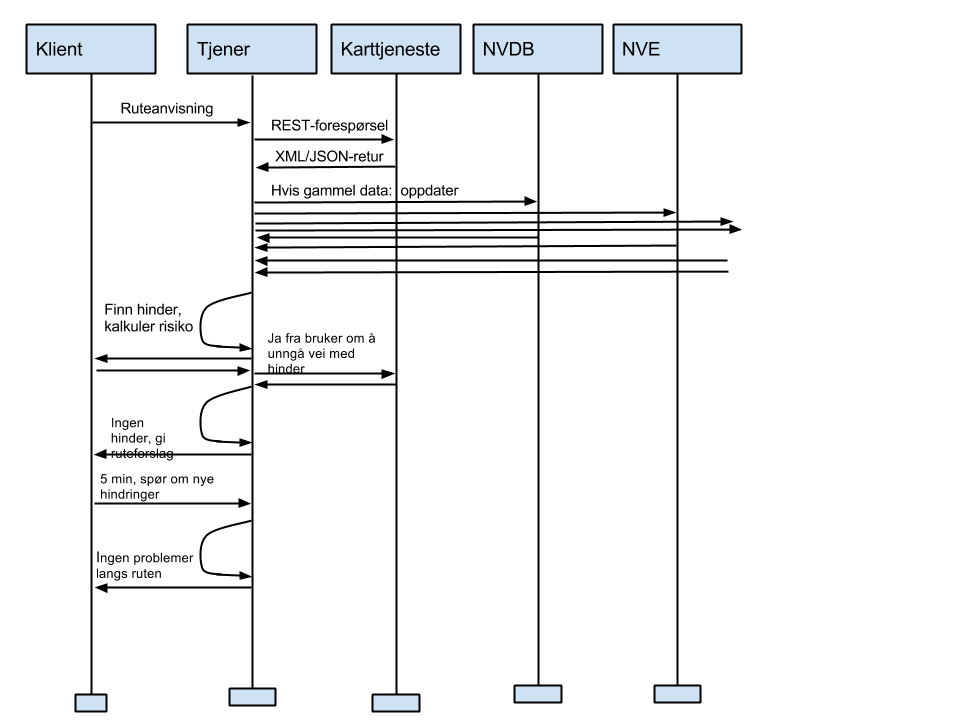
\includegraphics[scale=0.5]{figs/Sekvensdiagram.png}
\label{trafikkulykke}
\end{figure}

Dette sekvensdiagrammet illustrerer hvordan vi ser for oss at kommunikasjonen mellom leddene vil fungere. Applikasjonen vil sende en ruteforespørsel til en destinasjon, og tjeneren vil gi et gitt antall forslag som brukeren kan velge mellom. Dersom et hinder er oppdaget langs ruten spør man brukeren om han vil forsøke å unngå den veistrekningen. Tjeneren vil gi et nytt forslag dersom det er fornuftig, det vil være naturlig å sette en terskel for hvor lange omkjøringene vil være.
Tjeneren tar kontakt med andre tjenester dersom de mellomlagrede dataene er gamle nok. Hvor lang tid det går mellom hver spørring vil man se mer nøye på etter hvert som applikasjonen er klar for testing.
Underveis i kjøringen vil applikasjonen spørre om oppdateringer, og det vil være en god løsning å la dette skje oftere dersom brukeren kjører vekk fra den planlagte ruten.

Risikovurdering
Risikovurderingen i applikasjonen kan løses med variende grad av kompleksitet. Uten å utvikle prototyper er det vanskelig å undersøke hvilke løsninger som vil fungere, men vårt utgangspunkt i denne rapporten vil være en enkel metode som bruker beslutningstrær.

[DECISION TREE-diagram fra presentasjonen]

Tabellene med risikovurderinger gjort av en ekspert blir lagt opp som et beslutningstre som tjeneren vår går igjennom for å gjøre en totalvurdering. Vi har for eksempel værdata, rasfarevurderinger og historiske dyrepåkjørsler som kan overlappes for å avgjøre den totale risikoen i større regioner. Illustrasjonen under viser et eksempel hvor dårlig vær i et større område skaper “grønn” risiko, mens informasjon om rasfare og dyrepåkjørsler legges over disse for å skape “gul” eller “rød” risiko.

\begin{figure}[H]
\centering
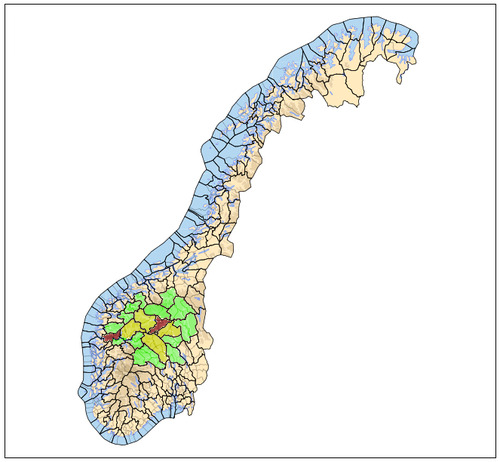
\includegraphics[scale=0.5]{figs/regioner.png}
\label{trafikkulykke}
\end{figure}

Denne regioninndelingen vil være mer presis i praksis, i eksempelet er inndelingen gjort for større regioner for illustrasjonshensikter.

Videre arbeid for å lage gode risikovurderinger kan ligge i å utforske Case-Based Reasoning som et virkemiddel, der maskinen mellomlagrer informasjon om mange ulykker hentet fra Norsk Vegdatabank, og sammenligner disse med informasjonen den har tilgjengelig om nåtiden for å vurdere risiko. Vi har observert at Vegvesenet lagrer mange detaljer for eksempelvis alvorlige trafikkulykker og dyrepåkjørsler, som vi kan se et eksempel på her.

\begin{figure}[H]
\centering
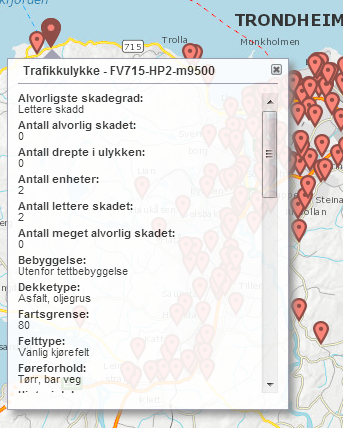
\includegraphics[scale=0.5]{figs/trafikkulykke.png}
\label{trafikkulykke}
\end{figure}

Vi har ikke anledning til å utvikle prototyper for dette og vil derfor ta utgangspunkt i beslutningstrær som et første stadie for en god risikovurderingsalgoritme.



\chapter{Oppsummering og konklusjon}
\label{sec:konklusjon}

\section{Samfunnsnytte}
\label{sec:samfunnsnytte}

 Applikasjonen vår kan bidra til å løse to store problemer relatert til samferdsel; trafikktetthet og ulykker. Trafikktetthetproblemet løses på to måter, både ved å foreslå veistrekninger med mindre kø og ved å foreslå omveier rundt ulykker som vil skape kø. Vi håper også at en applikasjon vil kunne ta i bruk metoder fra kunstig intelligens for å gjøre brukere oppmerksom på at de bør være mer på vakt i farlige områder, for eksempel ved å foreslå at de reduserer farten i utsatte områder.

Ved å omdirigere kjøretøy til mindre trafikkerte veier kan man forhåpentligvis redusere drivstofforbruk og CO2-utslipp, men andre kilder til forurensing kan potensielt øke i omfang, som for eksempel forekomst av svevestøv. Vi er også avhengig av at informasjon om trafikktetthet er oppdatert i tilnærmet sanntid for at brukerne ikke skal bli anbefalt å unngå ikke-eksisterende trafikk.

Ved å varsle brukeren om farlige områder vil man kunne redusere antall trafikkfarlige situasjoner som følge av at brukerne tar mer hensyn. Samtidig må vi være klar over muligheten for at brukerne vil ta mindre hensyn enn vanlig i områder som applikasjonen anser som mindre farlige. Man må også undersøke hvor mye risiko en slik applikasjon skaper i forhold til reduksjonen, da en applikasjon med varsling vil være distraherende for sjåføren.


\section{Videre arbeid}
\label{sec:varbeid}

I løpet av dette prosjektet har vi hovedsaklig jobbet med å kartlegge hvilke datakilder som er tilgjengelig i Norge og vurdert hvilke av dem som er best egnet for våre formål. Vi mener at funksjonaliteten vi har skissert for systemet vårt er realiserbar, selv om det kreves mye arbeid før det eventuelt kan settes i live. En sentral utfordringen i arbeidet videre blir å koordinere og tolke dataene som samles inn. Vi har gjort vurderinger rundt hvilke kilder som gir mest relevant informasjon, og har også gitt anbefalinger på grunnlag av hvor enkelt det er å integrere mot de enkelte kildene. Vi har derimot ikke gjennomført noen faktiske tester opp mot de enkelte API'ene, og det kan være utfordringer knyttet til hver enkelt kilde vi enda ikke vet om. 

Med tanke på å utelde en risikoprofil, må vi  enda større grad kunne skille mellom hvilken informasjon som er relevant eller ikke. Vi må også gjennomføre analyser av historiske data for å kunne komme frem til en passende model for å utlede risikoprofilen . Klarhet i hvordan intelligente metoder kan brukes i denne prosessen er også vesentlig.  Vi har diskutert det overfladiske og identifisert metoder som potensielt kan brukes, men vi har ikke testet det i praksis. Det gjenstår en god del arbeid for å komme frem til en ferdig modell. I tillegg vil det være en stor utfordring å samle inn en tilstrekkelig mengde treningsdata for å trene en intelligent algoritme. Vi har identifisert kilder til historisk informasjon, via NVDB, men er fremdeles usikker på hvordan denne informasjonen er lagret og hvilke parametre som inngår.

Vi har skissert en løsning på et komplisert problem. Selv om vi har kartlagt mange av elementene, er det på ingen måte en komplett systembeskrivelse. Det er nødvendig med videre undersøkelser for å belyse alle aspekter av systemet, i tllegg til dette kan det være viktige utfordringer vi har oversett. 

\section{Konklusjon}
\label{sec:konklusjon}

Vår problemstilling har vært å utrede tilgjengeligheten til relevante data for reisende langs veien, og hvordan man kan utnytte disse for å bedre informere brukerne om potensielle hindringer og risikofylte strekninger. Vi startet ved å undersøke eksisterende løsninger, og konkluderte med at disse var enten mindre aktuelle for bruk i Norge, eller for spesialiserte opp mot en enkelt funksjonalitet. Vi ønsket oss en komplett reiseassistent som inkluderte flere datakilder for å gi et så helhetlig bilde av trafikken som mulig, slik at man som bruker kun behøvde å forholde seg til én applikasjon.

Vårt arbeid har i hovedsak vært å utrede tilgjengeligheten av data i Norge, med tanke på hva slags data som eksisterer og hvor enkle disse dataene er å ta i bruk for applikasjonsutviklere. Vi har undersøkt hvordan tjenestene og datakildene kan knyttes sammen ved å utforme en systembeskrivelse, og basert på denne vurdert tilgjengeligheten.

Karttjenesten tilbyr all den funksjonaliteten vi krever, og den største utfordringen vil være potensielle unøyaktigheter i ruteplanleggeren, da spesielt med tanke på trafikkregler. Vi ønsket å kunne unngå trafikkulykker og veistrekninger med store mengder kø, og mens vegvesenet tilbyr informasjon som lar oss realisere førstnevnte, så er det fortsatt langt å gå når det kommer til å måle trafikkmengde i tilnærmet sanntid.

Et annet mål i applikasjonen er å vurdere risikoen i de veistrekningene som blir foreslått for brukeren. For å oppnå dette er vi avhengig av værdata, ras- og flomdata, informasjon om viltpåkjørsler, trafikkinformasjon om veiforhold og andre veimeldinger. Vi opplevde at værdata var tilfredsstillende, men at data om flom og ras fra NVE var mangelfullt, da de foreløpig kun tilbyr data om generell snøskredsfare for et fåtall store områder. De har derimot planer om å utvide dette tilbudet til jordskred- og flomfare i nåværende år. Underveis i dette prosjektet åpnet også vegvesenet sin databank NVDB, og vi fikk dermed tilgang til store mengder data som kunne benyttes for å utvikle risikoprofiler, da spesielt takket være tilgangen til historiske data om viltpåkjørsler og skred.

Konklusjonen vi har kommet til er at en applikasjon med funksjonaliteten vi ønsker oss ser ut til å være realiserbar i dag. For å oppnå dette er vi avhengige av en “klient-tjener”-modell for å realisere risikovurderingen av veistrekninger, og ser for oss at den største utfordringen blir å implementere de metodene innen kunstig intelligens som er foreslått.



\backmatter

\bibliographystyle{plain}
\bibliography{bibliography}

\addcontentsline{toc}{chapter}{Bibliography}
%\bibliography{bibtex/bibliography}


\chapter{Vedlegg}
\label{cha:appendices}


\end{document}
